\documentclass[dvipsnames]{beamer}
\usepackage[utf8]{inputenc}
\usepackage{listings}
\usepackage{comment}
\usepackage{soul}
%\usepackage{ulem}
\usepackage{subfig}
\setul{}{1pt}
\usepackage[oldenum, olditem]{paralist}
%allow even smaller text
\newcommand\tinytiny{\fontsize{4pt}{3}\selectfont}

\makeatletter
\let\old@lstKV@SwitchCases\lstKV@SwitchCases
\def\lstKV@SwitchCases#1#2#3{}
\makeatother
\usepackage{lstlinebgrd}
\makeatletter
\let\lstKV@SwitchCases\old@lstKV@SwitchCases

\lst@Key{numbers}{none}{%
    \def\lst@PlaceNumber{\lst@linebgrd}%
    \lstKV@SwitchCases{#1}%
    {none:\\%
     left:\def\lst@PlaceNumber{\llap{\normalfont
                \lst@numberstyle{\thelstnumber}\kern\lst@numbersep}\lst@linebgrd}\\%
     right:\def\lst@PlaceNumber{\rlap{\normalfont
                \kern\linewidth \kern\lst@numbersep
                \lst@numberstyle{\thelstnumber}}\lst@linebgrd}%
    }{\PackageError{Listings}{Numbers #1 unknown}\@ehc}}
\makeatother


\graphicspath{{logos/}}

\usepackage{tikz}
\graphicspath{{4_0/figures/}}
%disclaimer for Sandia. uncomment and the whole blob goes away @ b80c116300122
%\def\sandid{UPDATEME SAND2020-7755 PE}

% \title{Performance Portability with Kokkos}
\title{Kokkos 4.1 Release Briefing}

%BAD misuse of author field
\author{New Capabilities}


\usetheme{kokkos}

\newif\ifshort
\newif\ifmedium
\newif\iffull
\newif\ifnotoverview

\newcommand{\TutorialDirectory}{\texttt{Intro-Full}}
\newcommand{\ExerciseDirectory}[1]{\texttt{Exercises/#1/}}
\newcommand{\TutorialClone}{\texttt{Kokkos/kokkos-tutorials/\TutorialDirectory}}

\definecolor{darkgreen}{rgb}{0.0, 0.5, 0.0}
\definecolor{darkred}{rgb}{0.8, 0.0, 0.0}
\definecolor{orange}{rgb}{0.8, 0.33, 0.0}
\definecolor{purple}{rgb}{0.60, 0.20, 0.80}
\colorlet{bodyColor}{blue!20}
\colorlet{patternColor}{orange!30}
\colorlet{policyColor}{green!30}

% http://tex.stackexchange.com/questions/144448/color-a-text-line-in-a-code-lstlisting
\lstnewenvironment{code}[1][]%
{
  %with txfonts: OT1/txr/m/n/10
  %with default fonts: OT1/cmr/m/n/10
  %\fontfamily{cmr}\selectfont
  %\showthe\font
   \noindent
   \minipage{\linewidth}
   %\vspace{0.5\baselineskip}
   \lstset{mathescape, escapeinside={<@}{@>},
moredelim=**[is][{\btHL[fill=patternColor]}]{@pattern}{@pattern},
moredelim=**[is][{\btHL[fill=red!30]}]{@warning}{@warning},
moredelim=**[is][{\btHL[fill=policyColor]}]{@policy}{@policy},
moredelim=**[is][{\btHL[fill=bodyColor]}]{@body}{@body},
moredelim=**[is][{\btHL[fill=red!30]}]{@warning}{@warning},
moredelim=**[is][\color{black}]{@black}{@black},
moredelim=**[is][\color{blue}]{@blue}{@blue},
moredelim=**[is][\bf]{@bold}{@bold},
moredelim=**[is][\it]{@italic}{@italic},
moredelim=**[is][\color{boldblue}\bf]{@boldblue}{@boldblue},
moredelim=**[is][\color{red}]{@red}{@red},
moredelim=**[is][\color{green}]{@green}{@green},
moredelim=**[is][\color{gray}]{@gray}{@gray},
moredelim=**[is][\color{darkgreen}]{@darkgreen}{@darkgreen},
moredelim=**[is][\color{darkred}]{@darkred}{@darkred},
moredelim=**[is][\color{orange}]{@orange}{@orange},
moredelim=**[is][\color{purple}]{@purple}{@purple},
keywords={},
#1}
}
{
  \endminipage
  %\vspace{1.0\baselineskip}
}

\makeatletter
\newif\ifATOlinebackground
\lst@Key{linebackground}{\tiny}{\def\ATOlinebackground{#1}\global\ATOlinebackgroundtrue}
\makeatother

\lstnewenvironment{shell}[1][]{%
  \global\ATOlinebackgroundfalse
  \lstset{language=sh,%
    showstringspaces=false,
    aboveskip=0pt,
    frame=none,
    numbers=none,
    belowskip=2pt,
    breaklines=true,
    #1,
    }
  %\ifATOlinebackground
  \lstset{linebackgroundcolor={
    \ATOlinebackground
  }}
  %\fi
  }{}

\lstnewenvironment{cmake}[1][]{%
  \global\ATOlinebackgroundfalse
  \lstset{language=sh,%
    showstringspaces=false,
    aboveskip=0pt,
    frame=none,
    numbers=none,
    belowskip=2pt,
    breaklines=true,
    #1,
    }
  %\ifATOlinebackground
  \lstset{linebackgroundcolor={
    \ATOlinebackground
  }}
  %\fi
  }{}

\newcommand{\inlinecode}[1]{{\lstset{basicstyle=\ttfamily,keywordstyle={},showstringspaces=false}\lstinline$#1$}}
\newcommand{\inlineshell}[1]{{\lstset{basicstyle=\ttfamily,keywordstyle={},showstringspaces=false}\lstinline$#1$}}

\setbeamercolor{block title}{fg=white, bg=SandiaLightBlue}
\setbeamercolor{block body}{bg=lightgray}
\setbeamercolor{block title alerted}{fg=white, bg=SandiaRed}
\setbeamercolor{block body alerted}{bg=lightgray}



%\usepackage[texcoord,grid,gridunit=mm,gridcolor=red!10,subgridcolor=green!10]{eso-pic}
\usepackage[absolute,overlay]{textpos}





% http://tex.stackexchange.com/questions/8851/how-can-i-highlight-some-lines-from-source-code

\usepackage{pgf, pgffor}
\usepackage{listings}
\usepackage{lstlinebgrd} % see http://www.ctan.org/pkg/lstaddons

\makeatletter
%%%%%%%%%%%%%%%%%%%%%%%%%%%%%%%%%%%%%%%%%%%%%%%%%%%%%%%%%%%%%%%%%%%%%%%%%%%%%%
%
% \btIfInRange{number}{range list}{TRUE}{FALSE}
%
% Test in int number <number> is element of a (comma separated) list of ranges
% (such as: {1,3-5,7,10-12,14}) and processes <TRUE> or <FALSE> respectively

\newcount\bt@rangea
\newcount\bt@rangeb

\newcommand\btIfInRange[2]{%
    \global\let\bt@inrange\@secondoftwo%
    \edef\bt@rangelist{#2}%
    \foreach \range in \bt@rangelist {%
        \afterassignment\bt@getrangeb%
        \bt@rangea=0\range\relax%
        \pgfmathtruncatemacro\result{ ( #1 >= \bt@rangea) && (#1 <= \bt@rangeb) }%
        \ifnum\result=1\relax%
            \breakforeach%
            \global\let\bt@inrange\@firstoftwo%
        \fi%
    }%
    \bt@inrange%
}
\newcommand\bt@getrangeb{%
    \@ifnextchar\relax%
        {\bt@rangeb=\bt@rangea}%
        {\@getrangeb}%
}
\def\@getrangeb-#1\relax{%
    \ifx\relax#1\relax%
        \bt@rangeb=100000%   \maxdimen is too large for pgfmath
    \else%
        \bt@rangeb=#1\relax%
    \fi%
}

%%%%%%%%%%%%%%%%%%%%%%%%%%%%%%%%%%%%%%%%%%%%%%%%%%%%%%%%%%%%%%%%%%%%%%%%%%%%%%
%
% \btLstHL<overlay spec>{range list}
%
% TODO BUG: \btLstHL commands can not yet be accumulated if more than one overlay spec match.
%
\newcommand<>{\btLstHL}[2]{%
  \only#3{\btIfInRange{\value{lstnumber}}{#1}{\color{#2}\def\lst@linebgrdcmd{\color@block}}{\def\lst@linebgrdcmd####1####2####3{}}}%
}%
\makeatother






% http://tex.stackexchange.com/questions/15237/highlight-text-in-code-listing-while-also-keeping-syntax-highlighting
%\usepackage[T1]{fontenc}
%\usepackage{listings,xcolor,beramono}
\usepackage{tikz}

\makeatletter
\newenvironment{btHighlight}[1][]
{\begingroup\tikzset{bt@Highlight@par/.style={#1}}\begin{lrbox}{\@tempboxa}}
{\end{lrbox}\bt@HL@box[bt@Highlight@par]{\@tempboxa}\endgroup}

\newcommand\btHL[1][]{%
  \begin{btHighlight}[#1]\bgroup\aftergroup\bt@HL@endenv%
}
\def\bt@HL@endenv{%
  \end{btHighlight}%
  \egroup
}
\newcommand{\bt@HL@box}[2][]{%
  \tikz[#1]{%
    \pgfpathrectangle{\pgfpoint{1pt}{0pt}}{\pgfpoint{\wd #2}{\ht #2}}%
    \pgfusepath{use as bounding box}%
    \node[anchor=base west, fill=orange!30,outer sep=0pt,inner xsep=1pt, inner ysep=0pt, rounded corners=3pt, minimum height=\ht\strutbox+1pt,#1]{\raisebox{1pt}{\strut}\strut\usebox{#2}};
  }%
}
\makeatother



\usetikzlibrary{calc}
\usepackage{xparse}%  For \NewDocumentCommand

% tikzmark command, for shading over items
\newcommand{\tikzmark}[1]{\tikz[overlay,remember picture] \node (#1) {};}

\makeatletter
\NewDocumentCommand{\DrawBox}{s O{}}{%
    \tikz[overlay,remember picture]{
    \IfBooleanTF{#1}{%
        \coordinate (RightPoint) at ($(left |- right)+(\linewidth-\labelsep-\labelwidth,0.0)$);
    }{%
        \coordinate (RightPoint) at (right.east);
    }%
    \draw[red,#2]
      ($(left)+(-0.2em,0.9em)$) rectangle
      ($(RightPoint)+(0.2em,-0.3em)$);}
}

\NewDocumentCommand{\DrawBoxWide}{s O{}}{%
    \tikz[overlay,remember picture]{
    \IfBooleanTF{#1}{%
        \coordinate (RightPoint) at ($(left |- right)+(\linewidth-\labelsep-\labelwidth,0.0)$);
    }{%
        \coordinate (RightPoint) at (right.east);
    }%
    \draw[red,#2]
      ($(left)+(-\labelwidth,0.9em)$) rectangle
      ($(RightPoint)+(0.2em,-0.3em)$);}
}

\NewDocumentCommand{\DrawBoxWideBlack}{s O{}}{%
    \tikz[overlay,remember picture]{
    \IfBooleanTF{#1}{%
        \coordinate (RightPoint) at ($(left |- right)+(\linewidth-\labelsep-\labelwidth,0.0)$);
    }{%
        \coordinate (RightPoint) at (right.east);
    }%
    \draw[black,#2]
      ($(left)+(-\labelwidth,0.9em)$) rectangle
      ($(RightPoint)+(0.2em,-0.3em)$);}
}
\makeatother

\usetikzlibrary{positioning}

\usetikzlibrary{shapes}

\hypersetup{
    colorlinks=true,
    linkcolor=blue,
    filecolor=magenta,
    urlcolor=cyan,
}



\shorttrue
\mediumfalse
\fullfalse

\begin{document}

\begin{frame}
        \titlepage
\end{frame}


\begin{frame}[fragile]{Outline}

\textbf{4.1 Release Highlights}

    \begin{itemize}
      \item{Backend updates}
      \item{Build system updates}
      \item{Multiple Reducers for Nested Parallel Reduce}
      \item{Bit Manipulation}
      \item{UnorderedMap Insertion Operation Types}
      \item{Miscellaneous}
      \item{Deprecations and other breaking changes}
      \item{Kokkos on Compiler Explorer}
    \end{itemize}

\end{frame}

\begin{frame}{Find More}

\textbf{Online Resources}:

\begin{itemize}
        \item \url{https://github.com/kokkos}:
                \begin{itemize}
                        \item Primary Kokkos GitHub Organization
                \end{itemize}
        \item \url{https://github.com/kokkos/kokkos-tutorials/wiki/Kokkos-Lecture-Series}:
                \begin{itemize}
			\item{Slides, recording and Q\&A for the Full Lectures}
                \end{itemize}
        \item \url{https://kokkos.github.io/kokkos-core-wiki}:
                \begin{itemize}
                        \item Wiki including API reference
                \end{itemize}
        \item \url{https://kokkosteam.slack.com}:
                \begin{itemize}
                        \item Slack channel for Kokkos.
                        \item Please join: fastest way to get your questions answered.
                        \item Can whitelist domains, or invite individual people.
                \end{itemize}
\end{itemize}

\end{frame}

\begin{frame}[fragile]{Kokkos Usage}
  \textbf{Would like to strengthen community bonds and discoverability}

\vspace{10pt}
\textit{List of Applications and Libraries}
\begin{itemize}
\item Add your app to \url{https://github.com/kokkos/kokkos/issues/1950}
\item We are planning to add that to a Kokkos website.
\item Helps people discover each other when working on similar things.
\end{itemize}

\vspace{10pt}
\textit{GitHub Topics}
\begin{itemize}
\item Use \textit{kokkos} tag on your repos.
\item If you click on the topic you get a list of all projects on github with that topic.
\end{itemize}

\end{frame}

\begin{frame}[fragile]{Kokkos Topic}
  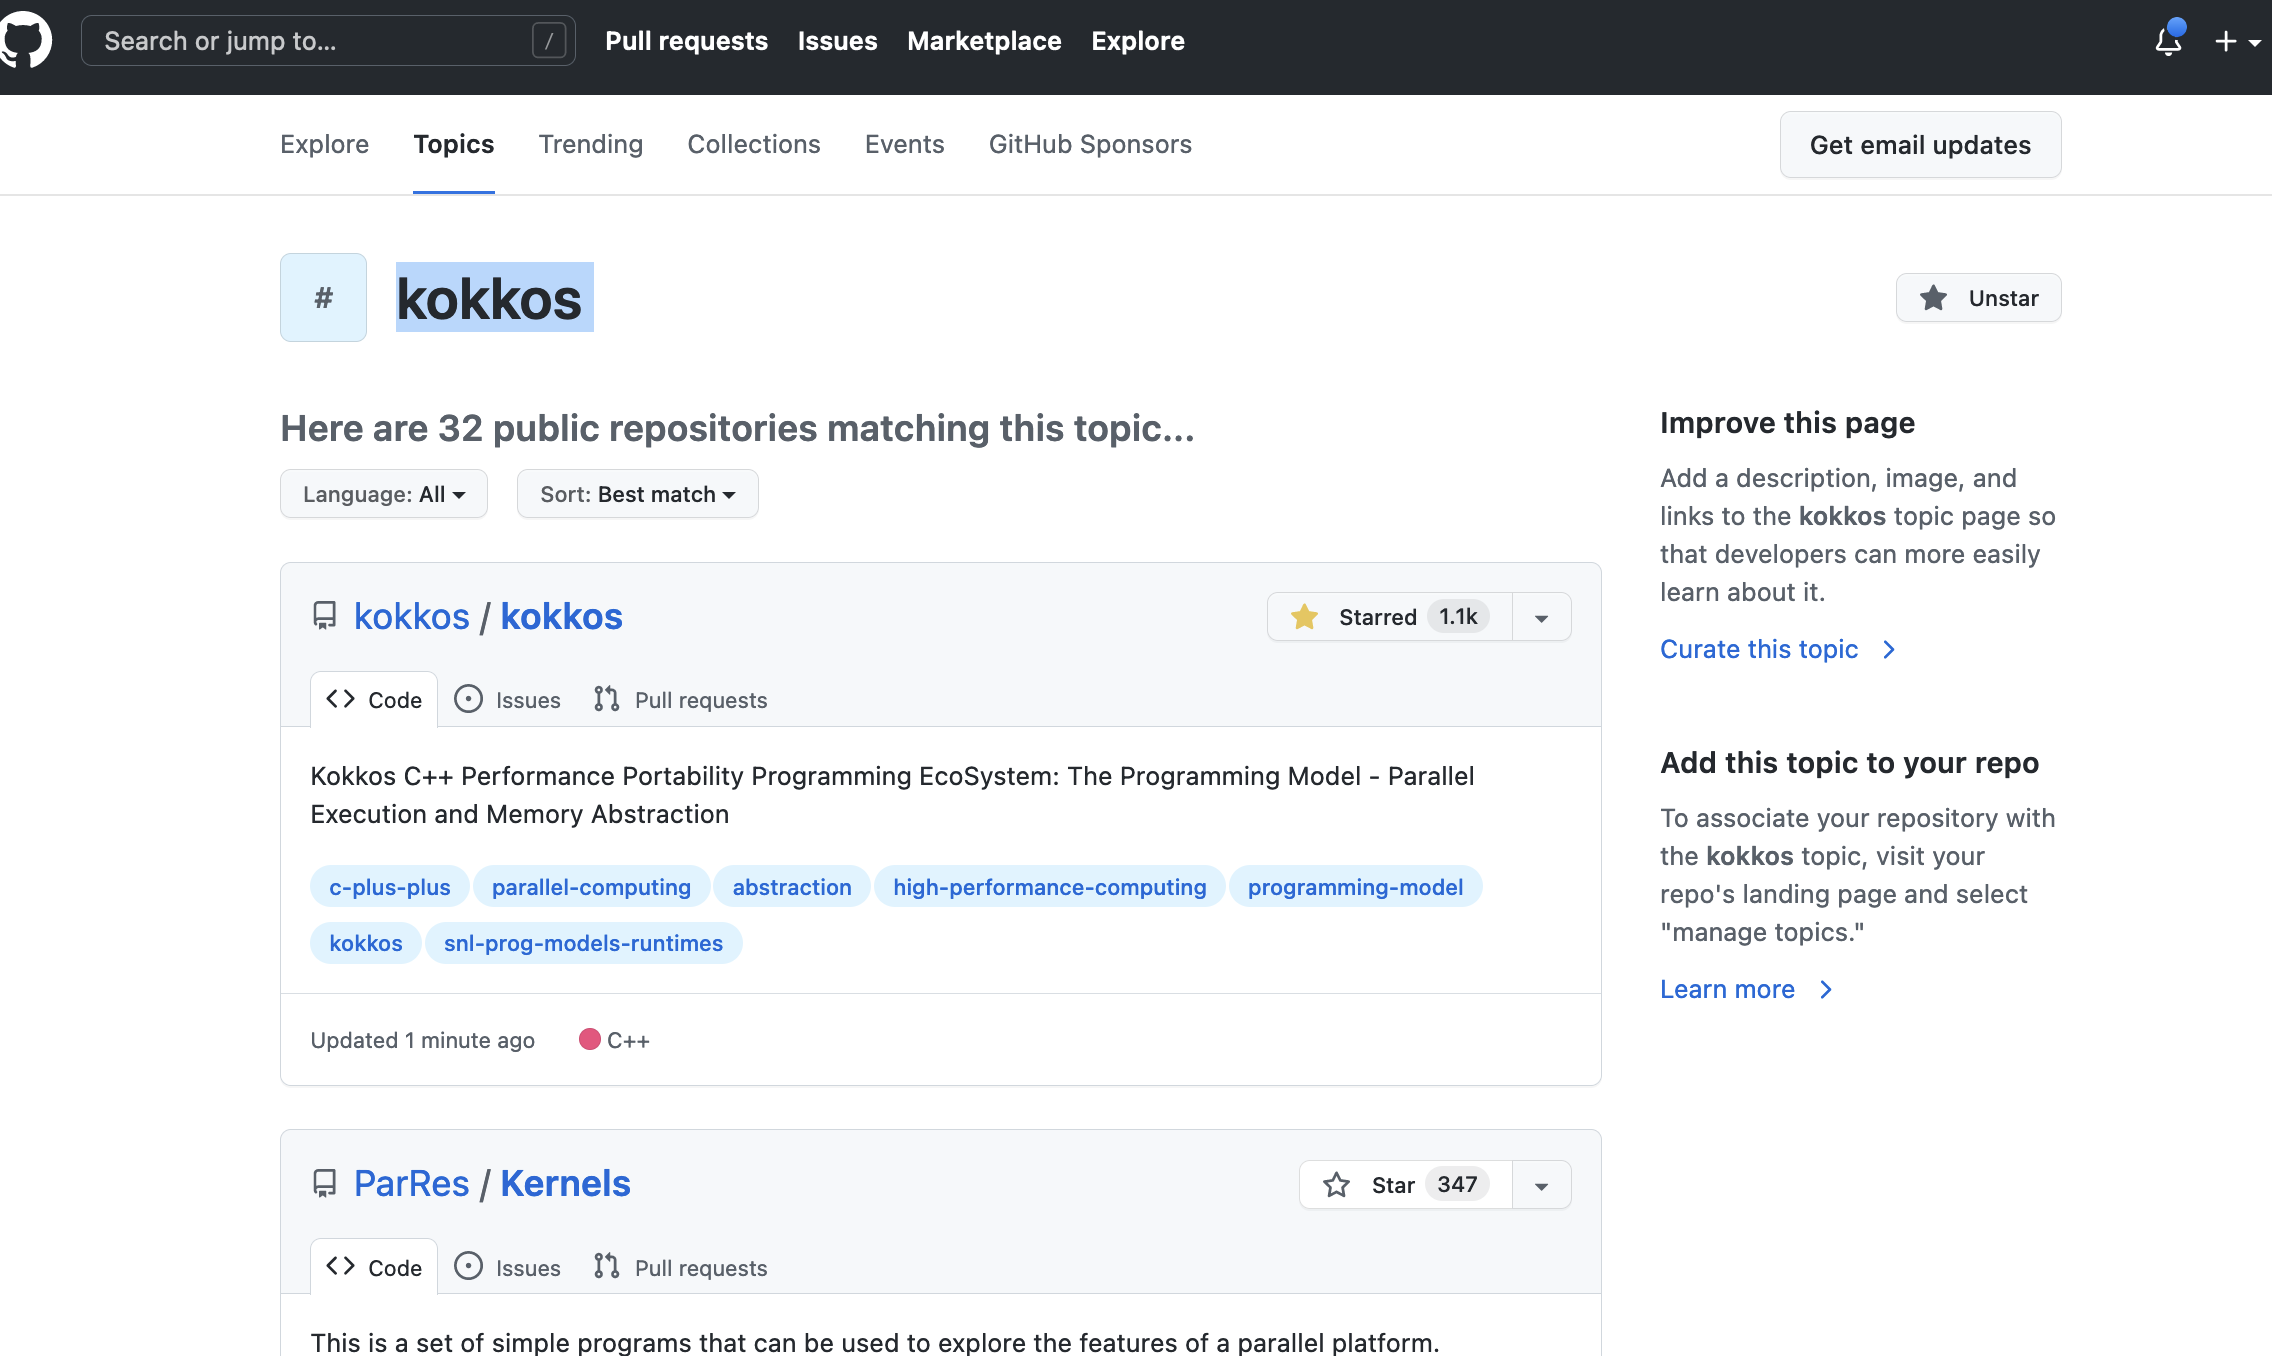
\includegraphics[width=0.9\textwidth]{3_7/kokkos-topic.png}
\end{frame}

\begin{frame}[fragile]{Kokkos user group meeting}
\begin{itemize}
\item We are considering organizing a multi-day in-person user group meeting
\item Likely in Albuquerque
\item postponed to early December time frame
\item Tentative content
   \begin{itemize}
   \item Updates from the Kokkos team (new features and planned work)
   \item User experiences: porting to AMD and Intel GPUs
   \item User experiences: performance portability studies
   \item Best practices (also user-provided)
   \item Students and Postdocs showcase
   \item Feedback and discussion session
   \end{itemize}
\end{itemize}
\end{frame}


%==========================================================================

\begin{frame}[fragile]

  {\Huge Backend Updates}

  \vspace{10pt}

  \textbf{Content:}
  \begin{itemize}
    \item Backend Updates Cuda
    \item Backend Updates HIP
    \item Backend Updates SYCL and OpenACC
  \end{itemize}

\end{frame}

%==========================================================================

\begin{frame}[fragile]{Backend Updates I}
\texttt{CUDA}
\begin{itemize}
    \item Fixed potential data race in \texttt{parallel\_reduce}
    \item Use \texttt{cudaMallocAsync} by default
    \item Bugfix when specifying non-default device ID while launching threads after initialization
    \item Deprecate \texttt{Cuda(cudaStream\_t,bool)} constructor
\end{itemize}
\end{frame}
\begin{frame}[fragile]{Backend updates II}
\texttt{HIP}
\begin{itemize}
    \item New naming convention:\\ \texttt{Kokkos\_ARCH\_VEGA90A} $\rightarrow$ \texttt{Kokkos\_ARCH\_AMD\_GFX90A}
    \item Add initial support for gfx942
    \item Add support for ROCM 5.5 and 5.6
    \item Improve reduction performance
    \item Fix potential data race in \texttt{HIP} \texttt{parallel\_reduce}
    \item Deprecate \texttt{HIP(hipStream\_t,bool)} constructor
    \item Add support for \texttt{Kokkos::Graph}
    \item Fix concurrency calculation
\end{itemize}
\end{frame}
\begin{frame}[fragile]{Backend Updates III}
\texttt{SYCL}
\begin{itemize}
    \item Enforce external \texttt{sycl::queues} to be in-order
    \item Make in-order \texttt{sycl::queues} the default via macro
    \item Improve reduction performance
    \item Allow using the \texttt{SYCL} execution space on AMD GPUs
    \item Allow sorting via native \texttt{oneDPL} to support \texttt{View}s with \texttt{stride=1}
\end{itemize}
\vfill
\texttt{OpenACC}
\begin{itemize}
    \item Add support for \texttt{clacc} compiler
\end{itemize}
\end{frame}

%==========================================================================



%==========================================================================


% Makefile and CMake support for C++23
% Update minimum compiler versions. (covered in earlier section)

\begin{frame}[fragile]{Build System Updates}
\textbf{C++ Standards Support}
\begin{itemize}
  \item \texttt{CMAKE\_CXX\_STANDARD=23} is supported
  \begin{itemize}
    \item \texttt{KOKKOS\_CXX\_STANDARD} for the Makefile
  \end{itemize}
  \item In CMake Kokkos will default to C++17 if no standard is specified
\end{itemize}
\end{frame}

%==========================================================================

% Let CMake determine OpenMP flags.
% Only add -latomic in generated GNU makefiles when OpenMPTarget backend is enabled

\begin{frame}[fragile]{Build System Updates}
\textbf{OpenMP and OpenMPTarget}
\begin{itemize}
  \item OpenMP flags are now determined by CMake's FindOpenMP
  \item Makefile: \texttt{libatomic} only linked in OpenMPTarget builds
\end{itemize}
\end{frame}

%==========================================================================

% Do not add -cuda to the link line with NVHPC compiler when the CUDA backend is not actually enabled
% Kokkos_ENABLE_CUDA_LAMBDA now ON by default with NVCC
% Fix enabling of relocatable device code when using CUDA as CMake language
% Fix cmake configuration with CUDA 12

\begin{frame}[fragile]{Build System Updates}
\textbf{CUDA}
\begin{itemize}
  \item \texttt{Kokkos\_ENABLE\_CUDA\_LAMBDA} set to \texttt{ON} by default
  \item Fixes to RDC flags when using CMake CUDA language
  \item Fixed CUDA 12 when using \texttt{nvcc\_wrapper} with CMake
  \item Fixes to using NVHPC as a compiler when CUDA is not enabled
\end{itemize}
\end{frame}

%==========================================================================



%==========================================================================

\begin{frame}[fragile]

  {\Huge Multiple Reducers for Nested Parallel Reduce}

  \vspace{10pt}

  \textbf{Content: Team-level parallel reduce with multiple reducers}
  \begin{itemize}
    \item Extended reducer capabilities in nested \texttt{parallel\_reduce}
    \item Allow multiple reductions in a single team \texttt{parallel\_reduce}
    \item Supported for \texttt{TeamThreadRange}, \texttt{ThreadVectorRange} and \texttt{TeamVectorRange} policies
    \begin{itemize}
      \item Not available for \texttt{TeamMDRangePolicies} for now
    \end{itemize}
  \end{itemize}

\end{frame}

%==========================================================================

\begin{frame}[fragile]{Multiple Reducers Interface}

\begin{code}[keywords={Team Parallel Reduce with Multiple Reducers}]
template <typename TeamPolicy, typename FunctorType,
          typename... ReducerArgument>
Kokkos::parallel_reduce(const TeamPolicy& policy,
                        const FunctorType& functor,
                        const ReducerArgument&... reducer);
\end{code}

\begin{code}[keywords={Team Parallel Reduce with Multiple Reduction Results}]
template <typename TeamPolicy, typename FunctorType,
          typename... ReducerArgumentNonConst>
Kokkos::parallel_reduce(const TeamPolicy& policy,
                        const FunctorType& functor,
                        ReducerArgumentNonConst&... reducer);

\end{code}

\begin{itemize}
  \item The number of reducers and the number of functor's reducer value arguments must match. 
\end{itemize}

\end{frame}

%==========================================================================

\begin{frame}[fragile]{Multiple Reducers Example}
  
  \begin{code}[keywords={TeamThreadMDRange}]
    
Kokkos::parallel_for(
  policy, KOKKOS_LAMBDA(team_member_type const& team) {
    /* ... */
    
    Kokkos::parallel_reduce(
      teamPolicy,
      [=](int& i, int& arg0, int& arg1, int& arg2, int& arg3) {
        /* ... */
      },
      result0, Kokkos::Prod<int>(result1),
      Kokkos::Max<int>(result2), result3);
  }
);

\end{code}

\end{frame}

%==========================================================================


%==========================================================================

\begin{frame}[fragile]

	{\Huge Bit Manipulation}

	\vspace{10pt}

	\textbf{Content:}
	\begin{itemize}
		\item \texttt{Kokkos::} equivalents for C++20/C++23 components to access, manipulate and process both individual bits and bit sequences
		      \begin{itemize}
		      	\item \texttt{bit\_cast}
		      	\item \texttt{byteswap}
		      	\item Integral powers of 2
		      	      \begin{itemize}
		      	      	\item \texttt{has\_single\_bit}, \texttt{bit\_ceil}, \texttt{bit\_floor}, \texttt{bit\_width}
		      	      \end{itemize}
		      	\item Rotating
		      	      \begin{itemize}
		      	      	\item \texttt{rotl}, \texttt{rotr}
		      	      \end{itemize}
		      	\item Counting
		      	      \begin{itemize}
		      	      	\item \texttt{countl\_zero}, \texttt{countl\_one}, \texttt{countr\_zero}, \texttt{countr\_one}, \texttt{popcount}
		      	      \end{itemize}
		      \end{itemize}
	\end{itemize}
\end{frame}

%==========================================================================

\begin{frame}[fragile]{bit\_cast}
	\texttt{\st{constexpr} To bit\_cast<To>(From const\& from) noexcept}
	\begin{itemize}
		\item Reinterpret the object representation of one type as that of another
		      \begin{itemize}
		      	\item \texttt{sizeof(From) == sizeof(To)}
		      	\item \texttt{From} must be trivially copyable
		      	\item \texttt{To} must be trivially copyable
		      \end{itemize}
		\item Not \texttt{constexpr} (differs from C++23 \texttt{std::bit\_cast})
	\end{itemize}
	\vfill
	\lstset {language=C++}
	\begin{lstlisting}
    double d1 = 19880124.0;
    auto  u64 = Kokkos::bit_cast<uint64_t>(d1);
    auto   d2 = Kokkos::bit_cast<double>(u64);
    
    assert(d1 == d2);
	\end{lstlisting}	
\end{frame}

%==========================================================================

\begin{frame}[fragile]{byteswap}
	\texttt{constexpr T byteswap(T value) noexcept}
	\begin{itemize}
		\item Reverses the bytes in the given integer value
		      \vfill
		\item \texttt{T} is an integral type
		      \begin{itemize}
		      	\item \texttt{bool}, \texttt{char}, \texttt{char8\_t}, \texttt{char16\_t}, \texttt{char32\_t}, \texttt{wchar\_t}, \texttt{short}, \texttt{int}, \texttt{long}, \texttt{long long}, clang \texttt{\_\_128} (but not gcc \texttt{\_\_128})
		      	      \begin{itemize}
		      	      	\item \texttt{signed} and \texttt{unsigned} integer types
		      	      \end{itemize}
		      \end{itemize}
	\end{itemize}
	\vfill
	\lstset {language=C++}
	\begin{lstlisting}
    int32_t i1 = 0xdeadbeef;
    auto    i2 = Kokkos::byteswap(i1);
    
    assert(i2 == 0xefbeadde);
	\end{lstlisting}	
\end{frame}

%==========================================================================

\begin{frame}[fragile]{Integral Powers of 2}
	\begin{itemize}
		\item \texttt{constexpr bool has\_single\_bit(T x) noexcept}
		      \begin {itemize}
		\item Checks if a number is an integral power of 2
	\end{itemize}
	\item \texttt{constexpr T bit\_ceil(T x) noexcept}
	\begin {itemize}
	\item Finds the smallest integral power of two not less than \texttt{x}
	\end{itemize}   
	\item \texttt{constexpr T bit\_floor(T x) noexcept}
	\begin{itemize}
		\item Finds the largest integral power of 2 not greater than \texttt{x}
	\end{itemize}
	\item \texttt{constexpr int bit\_width(T x) noexcept}
	\begin{itemize}
		\item Finds the smallest number of bits needed to represent \texttt{x}
	\end{itemize}
	\vfill
	\item \texttt{T} is an unsigned integer type
	\begin{itemize}
		\item \texttt{unsigned char}, \texttt{unsigned short}, \texttt{unsigned int}, \texttt{unsigned long}, \texttt{unsigned long long}
	\end{itemize}
	\end{itemize}
	\lstset {language=C++}
	\begin{lstlisting}
    uint64_t x = 5;  // 0b101
    assert(Kokkos::has_single_bit(x) == false);
    assert(Kokkos::bit_ceil(x) == 8); 
    assert(Kokkos::bit_floor(x) == 4); 
    assert(Kokkos::bit_width(x) == 3); 
	\end{lstlisting}	
\end{frame}

%==========================================================================

\begin{frame}[fragile]{Rotating}
	\begin{itemize}
		\item \texttt{constexpr T rotl(T x, int x) noexcept}
		      \begin {itemize}
		\item Computes the result of a bitwise left-rotation
	\end{itemize}
	\item \texttt{constexpr T rotr(T x, int x) noexcept}
	\begin {itemize}
	\item Computes the result of a bitwise right-rotation
	\end{itemize}
	\vfill
	\item \texttt{T} is an unsigned integer type
	\end{itemize}
	\vfill
	\lstset {language=C++}
	\begin{lstlisting}
    uint16_t i16 = 0b1001110000111001;
    assert(Kokkos::rotl(i16, 2) == 0b0111000011100110);
    assert(Kokkos::rotr(i16, 3) == 0b0011001110000111);
	\end{lstlisting}	
\end{frame}

%==========================================================================

\begin{frame}[fragile]{Counting}
	\begin{itemize}
		\item \texttt{constexpr int countl\_zero(T x) noexcept}
		      \begin {itemize}
		\item Count the number of consecutive 0 bits, starting from the most significant bit
	\end{itemize}
	\item \texttt{constexpr int countl\_one(T x) noexcept}
	\begin {itemize}
	\item Count the number of consecutive 1 bits, starting from the most significant bit
	\end{itemize}
	\item \texttt{constexpr int countr\_zero(T x) noexcept}
	\begin {itemize}
	\item Count the number of consecutive 0 bits, starting from the least significant bit
	\end{itemize}
	\item \texttt{constexpr int countr\_one(T x) noexcept}
	\begin {itemize}
	\item Count the number of consecutive 1 bits, starting from the least significant bit
	\end{itemize}
	\item \texttt{constexpr int popcount(T x) noexcept}
	\begin {itemize}
	\item Count the number of 1 bits in an unsigned integer
	\end{itemize}
	\vfill
	\item \texttt{T} is an unsigned integer type
	\end{itemize}
\end{frame}

%==========================================================================

\begin{frame}[fragile]{Counting}
	\lstset {language=C++}
	\begin{lstlisting}
    uint16_t bits = 0b1111101000110100;

    assert(Kokkos::countl_zero(bits) == 0);
    assert(Kokkos::countl_one(bits)  == 5);
    assert(Kokkos::countr_zero(bits) == 2);
    assert(Kokkos::countr_one(bits)  == 0);
    assert(Kokkos::popcount(bits)    == 9);
	\end{lstlisting}
\end{frame}

%==========================================================================

\begin{frame}[fragile]{Builtins}
	\begin{itemize}
		\item In \texttt{namespace Kokkos::Experimental::}
		\item Not \texttt{constexpr}
		\item Directly call the compiler builtin version, if beneficial
		      \vfill
		\item \texttt{bit\_cast\_builtin}
		\item \texttt{byteswap\_builtin}
		\item Integral powers of 2
		      \begin{itemize}
                         \item \texttt{has\_single\_bit\_builtin}, \texttt{bit\_ceil\_builtin}, \texttt{bit\_floor\_builtin}, \texttt{bit\_width\_builtin}
		      \end{itemize}
		\item Rotating
		      \begin{itemize}
                         \item \texttt{rotl\_builtin}, \texttt{rotr\_builtin}
		      \end{itemize}
		\item Counting
		      \begin{itemize}
                         \item \texttt{countl\_zero\_builtin}, \texttt{countl\_one\_builtin}, \texttt{countr\_zero\_builtin}, \texttt{countr\_one\_builtin}, \texttt{popcount\_builtin}
		      \end{itemize}
	\end{itemize}
\end{frame}

%==========================================================================


%==========================================================================

\begin{frame}[fragile]

  {\Huge UnorderedMap Insertion Operation Types}

  \vspace{10pt}

  \textbf{Content: Extended UnorderedMap insertion behavior}
  \begin{itemize}
    \item Default behavior is to insert a key, value pair exactly once
    \item Maintain default behavior via operation type \texttt{NoOp}
    \item Allow existing key, value pairs to be accumulated into via operation type \texttt{AtomicAdd}
  \end{itemize}

\end{frame}

%==========================================================================

\begin{frame}[fragile]{UnorderedMap Insertion Interface}

\begin{code}[keywords={UnorderedMap Insertion Operation Types}]
template <class ValueTypeView, class ValuesIdxType>
struct UnorderedMapInsertOpTypes {
  using value_type = typename ValueTypeView::non_const_value_type;
  struct NoOp {
    void op(ValueTypeView, ValuesIdxType, const value_type);
  };
  struct AtomicAdd {
    void op(ValueTypeView values, ValuesIdxType values_idx,
            const value_type v);
  };
};
\end{code}

\begin{code}[keywords={UnorderedMap Insertion Interface}]
template <typename InsertOpType = default_op_type>
insert_result insert(key_type const &key,
                     impl_value_type const &value,
                     InsertOpType arg_insert_op = InsertOpType());
\end{code}

\begin{itemize}
  \item For other use-cases, more operation types can be added to \texttt{UnorderedMapInsertOpTypes}
\end{itemize}

\end{frame}

%==========================================================================

\begin{frame}[fragile]{UnorderedMap AtomicAdd Operation Type Example}
  
  \begin{code}[keywords={UnorderedMap Insertion Example}]

using map_op_type    
  = Kokkos::UnorderedMapInsertOpTypes<value_view_type, size_type>;
using atomic_add_type = typename map_op_type::AtomicAdd;
atomic_add_type atomic_add;
parallel_for(N, KOKKOS_LAMBDA (uint32_t i) {
  map.insert(i, values(i), atomic_add);
});

\end{code}

\end{frame}

%==========================================================================



\begin{frame}[fragile]{Miscellaneous}
\begin{itemize}
  \item Add \texttt{Kokkos::Profiling::ScopedRegion}
    \begin{code}	
     double myfunction()
     {
      Kokkos::Profiling::ScopedRegion region("foo");
      if (..)
        return bar;
      else
        return eval();
     }
    \end{code}
  \item Add support for \texttt{View::rank[\_dynamic]()}
  \item Detect incompatible relocatable device code mode to prevent ODR violations
  \item Add (experimental) support for 32-bit Darwin and PPC
  \item Add missing half and bhalf specialization of the infinity numeric trait
\end{itemize}
\end{frame}

\begin{frame}[fragile]{Miscellaneous}
\begin{itemize}
  \item Add \texttt{is\_dual\_view} trait and align template parameters with regular view
  \item Allow templated functors in \texttt{parallel\_for},
  \texttt{parallel\_reduce}, and \texttt{parallel\_scan}
  \item Define \texttt{KOKKOS\_COMPILER\_INTEL\_LLVM} and only define at most one
  \texttt{KOKKOS\_COMPILER*} macro
\end{itemize}
\end{frame}


%==========================================================================

\begin{frame}[fragile]

  {\Huge Deprecations}
  
    \vspace{10pt}

\end{frame}

\begin{frame}[fragile]{Deprecations}
\begin{itemize}
\item Deprecated allocation step inside \texttt{deep\_copy(UnorderedMap,UnorderedMap)}
  \begin{itemize}
    \item[] Maps now must have the same capacity to \texttt{deep\_copy}
  \end{itemize}
\item Deprecated implicit conversions of integers to \texttt{ChunkSize}
\begin{itemize}
  \item[] Behavior only introduced in 4.3
\end{itemize}
\item Deprecated implicit conversions to all execution spaces
\end{itemize}

\end{frame}

%==========================================================================

\begin{frame}[fragile]{Deprecate \texttt{Array<...,Proxy>} Argument}
\begin {itemize}
\item Deprecated trailing \texttt{Proxy} template argument in \texttt{Kokkos::Array}
\begin{code}
// DEPRECATED
// template <typename T = void,
//           size_t N = KOKKOS_INVALID_INDEX,
//           typename Proxy = void>
template <typename T, size_t N>
struct Array { /* ... */ };
\end{code}
  \begin{itemize}
    \item Deprecates \textit{non-owning, dynamically sized} \texttt{contiguous/strided} functionality
    \item More in line with (always) \textit{owning} \& \textit{statically sized} \texttt{std::array}
  \end{itemize}
\end{itemize}
\end{frame}

%==========================================================================

\begin{frame}[fragile]{Deprecate \texttt{is\_layouttiled}}
\begin {itemize}
\item Removed \texttt{Kokkos::Experimental::LayoutTiled} class template
  \begin{itemize}
  \item Never useable
  \end{itemize}
\item Deprecated \texttt{is\_layouttiled} trait
  \begin{itemize}
  \item Not useful, but no rush to remove it
  \end{itemize}
\item Deprecated \texttt{Kokkos::layout\_iterate\_type\_selector}
  \begin{itemize}
  \item Not useful outside of Kokkos implementation
  \end{itemize}
\end{itemize}
\end{frame}

%==========================================================================
\begin{frame}[fragile]{Deprecate \texttt{pair<T,void>}}
\begin {itemize}
\item Deprecated specialization of \texttt{Kokkos::pair} for a single element
\begin{code}
// DEPRECATED
// template <typename T>
// struct pair<T, void> { /* ... */ };
\end{code}
  \begin{itemize}
  \item Never supported in \texttt{std::pair}
  \item Never documented
  \item Never tested
  \item No known usage
  \end{itemize}
\end{itemize}
\end{frame}

%==========================================================================


%==========================================================================

\begin{frame}[fragile]

  \vspace{10pt}

  \textbf{How to Get Your Fixes and Features into Kokkos}
  \newline
  \begin{itemize}
    \item Fork the Kokkos repo (https://github.com/kokkos/kokkos)
    \item Make topic branch from \textit{develop} for your code
    \item Add tests for your code
    \item Create a Pull Request (PR) on the main project \textit{develop}
    \item Update the documentation (https://github.com/kokkos/kokkos-core-wiki) if your code changes the API
    \item Get in touch if you have any questions (https://kokkosteam.slack.com)
  \end{itemize}

\end{frame}

%==========================================================================

\end{document}


